\section{Versuchsaufbau}
\label{sec:Versuchsaufbau}

\begin{figure}
	\centering
	\begin{subfigure}[b]{0.28\textwidth}
		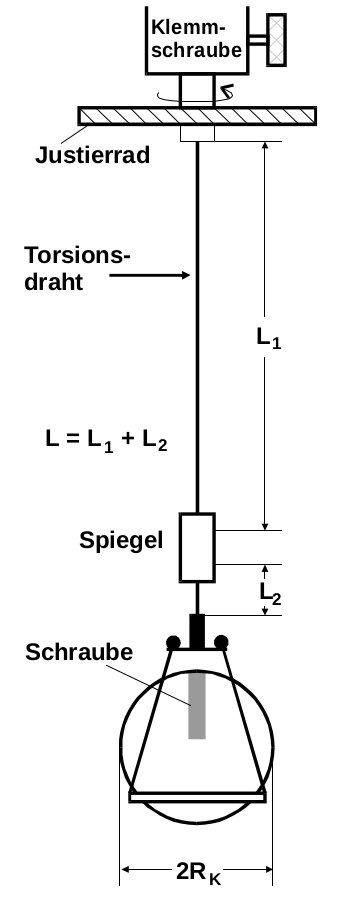
\includegraphics[width=\textwidth]{Bilder/aufbauallgemein.png}
		\caption{Prinzipieller Aufbau des schwingfähigen Systems}
		\label{fig:pendel}
	\end{subfigure}
	\begin{subfigure}[b]{0.66\textwidth}
		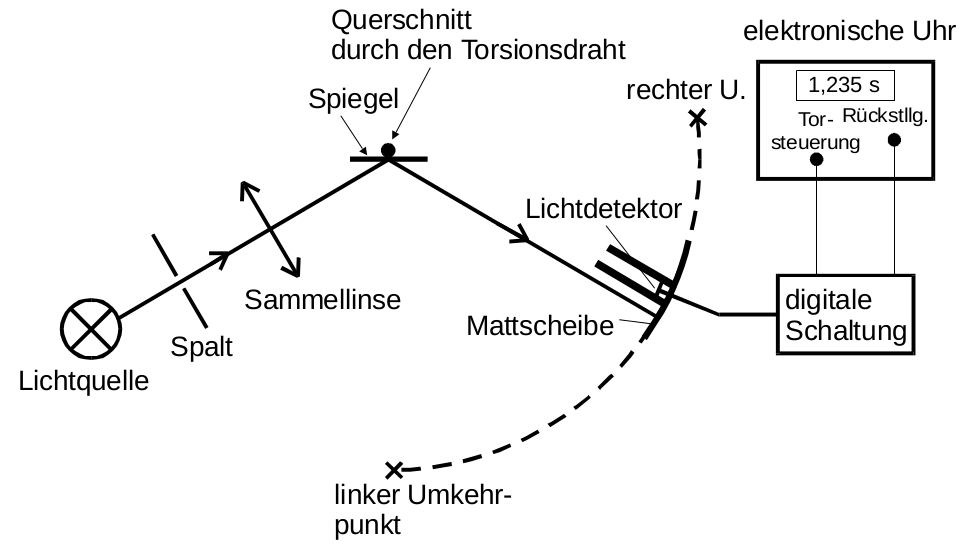
\includegraphics[width=\textwidth]{Bilder/spiegelding.png}
		\caption{Schematische Aufsicht der Signalweitergabe an den Zeitmesser.}
		\label{fig:licht}
	\end{subfigure}
	\caption{Versuchsaufbau zur Untersuchung der Schwingungsdauer des Drehschwingers. \cite{Anleitung}}
	\label{fig:aufbau_schwinger}
\end{figure}
In Abbildung \ref{fig:pendel} ist die prinzipielle Versuchsanordnung dargestellt. Es handelt sich hierbei um ein Pendel, welches in der Lage ist, Drehschwingungen auszuführen. Der Pendeldraht ist hierbei aus einem zunächst unbekannten Metall, dessen elastische Konstanten über die Periodendauer $T$ der Drehschwingung bestimmt werden. In der Kugelmasse am Pendel befindet sich zudem ein Magnet, dessen Ausrichtung anhand einer Schraube gekennzeichnet ist. Dieser wird, wie in der Durchführung beschrieben, je nach Messaufgabe, verschieden ausgerichtet.
Zur genauen Messung der Periodendauer $T$ ist ein kleiner Spiegel knapp oberhalb der Pendelmasse am Draht angebracht.
Über diesen wird, wie in Abbildung \ref{fig:licht}, ein gebündelter Lichtstrahl bei bestimmten Auslenkungen des Drehschwingers so reflektiert, dass er auf eine Photodiode trifft.
Die Photodiode sendet, wenn der Lichtstrahl sie überstreicht, ein Signal über die digitale Schaltung an die elektronische Stoppuhr.
Die digitale Schaltung ist so realisiert, dass beim ersten Überstreichen des Lichtstrahls über die Photodiode die Stoppuhr gestartet wird.
Das zweite Signal wird ignoriert. Dies wird realisiert über die Speicherfunktion eines RS-Flip-Flop und darüber, dass die Stoppuhr die fallende Flanke triggert.
Beim dritten Signal wird die Stoppuhr gestoppt (es wurde somit eine volle Periode gemessen) und beim vierten Signal wird die Stoppuhr zurückgesetzt.
Dies wird erreicht über die Speicherfunktion eines zweiten RS-Flip-Flops sowie eines AND-Gatters. Mit dem fünften Signal ist die Schaltung im gleichen Zustand wie beim ersten Signal, sodass die nächste Periode direkt anschließend gemessen werden kann.

\FloatBarrier
\subsection{Magnetisches Moment eines Permanentmagneten}

\begin{figure}
	\centering
	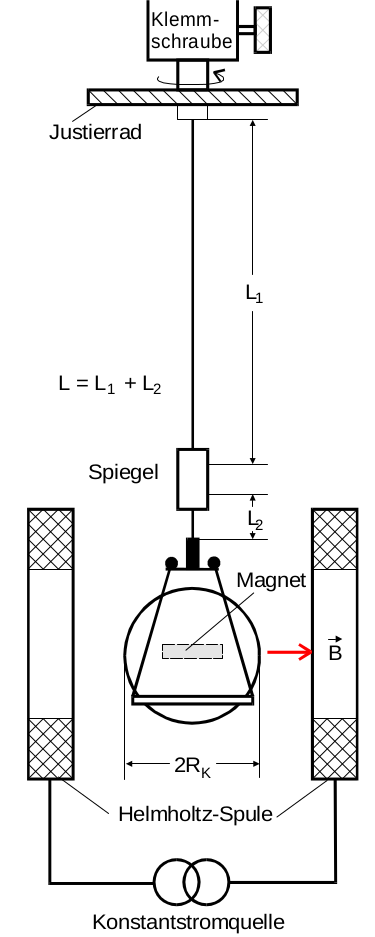
\includegraphics[width=0.3\textwidth]{Bilder/helmholtz.png}
	\caption{Versuchsaufbau zur Untersuchung des magnetischen Moments eines Permanentmagneten. \cite{Anleitung}}
	\label{fig:helmholtz}
\end{figure}
Zur Bestimmung des magnetischen Moments wird der Versuchsaufbau um ein Helmholtzspulenpaar, wie in Abbildung \refeq{fig:helmholtz} gezeigt, erweitert.
